\section{Localizzazione di autovalori}

Vogliamo ora studiare dei teoremi per \emph{localizzare} gli autovalori di una matrice $\Mat{\C, n, n}$, ovvero per individuare in quali regioni del piano complesso essi sono compresi.

Questo può essere utile per molte applicazioni: ad esempio ricordiamo che \[
    \norm{A}_2 = \sqrt{\rho\parens[\big]{AA\trans}},
\] dove $\rho(M)$ è definito come il massimo degli autovalori di $M$. Sarebbe quindi comodo avere un modo per determinare velocemente gli autovalori di una matrice $M$, o comunque approssimarli.

\begin{theorem}{Teorema di Hirsch}{hirsch}
    Sia $A \in \Mat{\C, n, n}$ e sia $\norm$ una norma matriciale indotta. Allora per ogni $\lambda \in \C$ autovalore di $A$ si ha \[
        \abs*{\lambda} \leq \norm{A}.
    \] Questo in particolare ci dice che \[
        \rho(A) \leq \norm{A}.
    \]
\end{theorem}

Da un punto di vista grafico questo significa che rappresentando gli autovalori di $A$ nel piano complesso, essi sono tutti contenuti in un cerchio che ha raggio $\norm{A}$, per qualunque norma matriciale indotta.

\begin{center}
    \tikzsetnextfilename{hirsch_exmpl}
    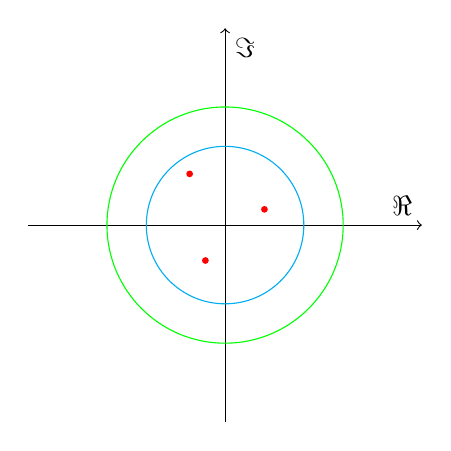
\begin{tikzpicture}[scale=.5]
        % Axis
        \draw [->] (-5,0) -- (5,0) node [above left]  {$\Re$};
        \draw [->] (0,-5) -- (0,5) node [below right] {$\Im$};

        \draw[cyan] (0,0) circle (2);
        \draw[green] (0,0) circle (3);
        
        \filldraw[red] (1,0.4) circle (2pt);
        \filldraw[red] (-0.5, -0.9) circle (2pt);
        \filldraw[red] (-0.9, 1.3) circle (2pt);
    \end{tikzpicture}
\end{center}

Dimostriamo ora il \nameref{th:hirsch}.
\begin{proof}
    Per definizione di autovalore deve esistere un vettore $\vec x \in \C^n$, $\vec x \neq \vec 0$ tale che \[
        A\vec x = \lambda\vec x.
    \] Sia $\norm$ la norma vettoriale che induce la norma matriciale che stiamo considerando: allora \[
        \abs{\lambda} \cdot \norm{\vec x}
        = \norm{\lambda\vec x}
        = \norm{A\vec x}
        \leq \norm{A} \cdot \norm{x}.
    \]

    Siccome $\vec x \neq \vec 0$ si ha che $\norm{\vec x} > 0$, dunque dividendo entrambi i membri per $\norm{\vec x}$ otteniamo \[
        \abs{\lambda} \leq \norm{A}. \qedhere
    \]
\end{proof}

\subsection{Teoremi di Gershgorin}

Vogliamo ora localizzare ancora più precisamente gli autovalori di una matrice.

\begin{definition}{Cerchi di Gershgorin}{}
    Sia $A \in \Mat{\C, n, n}$. Per ogni $1 \leq i \leq n$ definiamo l'$i$-esimo \strong{cerchio di Gershgorin} come l'insieme \[
        K_i \deq \set*{z \in \C \given \abs*{z - a_{ii}} \leq \sum_{j=1, j\neq i}^n \abs{a_{ij}}}.
    \]
\end{definition}

L'$i$-esimo cerchio è quindi dato da tutti i punti la cui distanza da $a_{ii}$ (l'elemento della diagonale nella $i$-esima riga) è minore della somma di tutti gli elementi dell'$i$-esima riga, escluso l'elemento della diagonale. Segue quindi che \begin{itemize}
    \item $a_{ii}$ rappresenta il \emph{centro} del cerchio $K_i$;
    \item $\sum_{j = 1, j\neq i}^n \abs{a_{ij}}$, ovvero la somma degli elementi dell'$i$-esima riga escluso $a_{ii}$, è il \emph{raggio} del cerchio.   
\end{itemize}

\begin{example}
    Consideriamo la matrice \[
        A = \begin{pmatrix}
            -1 & -1 & 0 \\
            -1 & 2  & 1 \\
            2  & 0  & 3 \\
        \end{pmatrix}.
    \] I corrispondenti cerchi di Gershgorin sono \begin{align}
        &K_1 = \set*{z \in \C \given \abs*{z + 1} \leq \abs{-1} + \abs{0} = 1} \\
        &K_2 = \set*{z \in \C \given \abs*{z - 2} \leq \abs{-1} + \abs{1} = 2} \\
        &K_3 = \set*{z \in \C \given \abs*{z - 3} \leq \abs{2} + \abs{0} = 2}.
    \end{align}

    Rappresentiamoli nel piano complesso:
    \begin{center}
        \tikzsetnextfilename{gershgorin_exmpl1}
        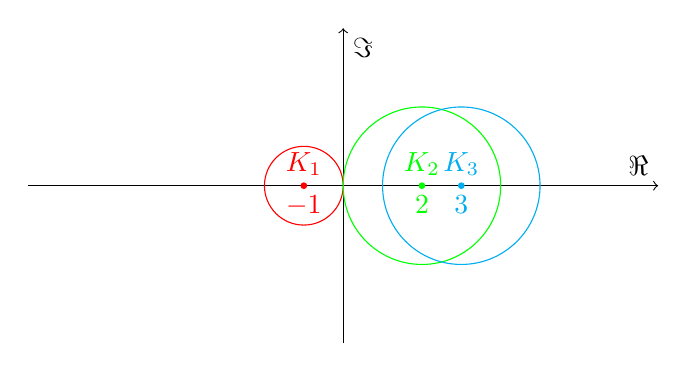
\begin{tikzpicture}[scale=.5]
            % Axis
            \draw [->] (-8,0) -- (8,0) node [above left]  {$\Re$};
            \draw [->] (0,-4) -- (0,4) node [below right] {$\Im$};

            \draw[red] (-1,0)  circle (1) node[above] {$K_1$}; % [$K_1$];
            \draw[green] (2,0) circle (2) node[above] {$K_2$}; % [$K_2$];
            \draw[cyan] (3,0)  circle (2) node[above] {$K_3$}; % [$K_3$];

            \filldraw[red] (-1,0)  node[below] {$-1$} circle (2pt); % [$K_1$];
            \filldraw[green] (2,0) node[below] {$2$}  circle (2pt); % [$K_2$];
            \filldraw[cyan] (3,0)  node[below] {$3$}  circle (2pt); % [$K_3$];
        \end{tikzpicture}
    \end{center}
\end{example}

\begin{theorem}
    {Primo Teorema di Gershgorin}
    {gershgorin_1}
    Sia $A \in \Mat{\C, n, n}$ e $\K_i$ i suoi cerchi di Gershgorin. Allora per ogni $\lambda \in \C$ autovalore di $A$ si ha \[
        \lambda \in \bigunion_{i=1}^n K_i.
    \]
\end{theorem}
\begin{proof}
    Sia $\lambda \in \C$ un autovalore di $A$, ovvero tale che esiste $\vec x \in \C^n$, $\vec x \neq \vec 0$ tale che $A\vec x = \lambda\vec x$. Scrivendo la matrice e i vettori per esteso questo equivale a \[
        \begin{pmatrix}
            a_{11} &\dots  &a_{1n} \\
            \vdots &\ddots &\vdots \\
            a_{n1} &\dots  &a_{nn} \\
        \end{pmatrix} \begin{pmatrix}
            x_1 \\ \vdots \\ x_n
        \end{pmatrix} = \lambda \begin{pmatrix}
            x_1 \\ \vdots \\ x_n
        \end{pmatrix} = \begin{pmatrix}
            \lambda x_1 \\ \vdots \\ \lambda x_n    
        \end{pmatrix}.
    \] Svolgendo il prodotto otteniamo che per ogni riga $1 \leq i \leq n$ vale che \[
        \begin{pmatrix}
            a_{i1} &\dots a_{in}
        \end{pmatrix} \begin{pmatrix}
            x_1 \\ \vdots \\ x_n
        \end{pmatrix} = a_{i1}x_1 + \dots + a_{in}x_n 
        = \sum_{j=1}^n a_{ij}x_j
        = \lambda x_i.
    \] Portando fuori dalla sommatoria il termine corrispondente a $j = i$ otteniamo \begin{align*}
        &\parens*{\sum_{j=1, j\neq i}^n a_{ij}x_j} + a_{ii}x_i = \lambda x_i\\
        \iff {}&\sum_{j=1, j\neq i}^n a_{ij}x_j =  \lambda x_i - a_{ii}x_i
    \end{align*} sempre per ogni $i = 1, \dots, n$.
    
    Sia ora $p$ l'indice per cui \[
        \abs*{x_p} = \norm{\vec x}_\infty = \max_{1 \leq i \leq n} \abs*{x_i},
    \] ovvero $p$ è l'indice della componente di modulo massimo. 
    Siccome $\vec x \neq \vec 0$ sicuramente c'è almeno una componente diversa da $0$, dunque $\abs*{x_p} > 0$. 
    
    Riscrivo quindi l'ultima equazione nel caso particolare di $i = p$: \[
        \sum_{j=1, j\neq p}^n a_{pj}x_j =  \lambda x_p - a_{pp}x_p
    \] che passando ai moduli diventa \[
        \abs*{\lambda - a_{pp}}\cdot \abs*{x_p} 
        = \abs*{\sum_{j=1, j\neq p}^n a_{pj}x_j} 
        \leq \sum_{j=1, j\neq p}^n \abs*{a_{pj}} \cdot \abs*{x_j},
    \] dove all'ultimo passaggio abbiamo usato la disuguaglianza triangolare dei moduli.

    Dividendo per $\abs*{x_p}$ (siccome è sempre strettamente maggiore di $0$) si ha \begin{align*}
        \abs*{\lambda - a_{pp}} 
        &\leq \frac{1}{\abs*{x_p}}\sum_{j=1, j\neq p}^n \abs*{a_{pj}} \cdot \abs*{x_j}\\
        &= \sum_{j=1, j\neq p}^n \abs*{a_{pj}} \cdot \frac{\abs*{x_j}}{\abs*{x_p}}.
        \intertext{Osserviamo ora che $\frac{\abs*{x_j}}{\abs*{x_p}}$ è sempre minore o uguale a $1$: infatti $x_p$ è la componente di modulo massimo, dunque il numeratore della frazione è sempre minore o uguale al denominatore. Si ha quindi}
        \abs*{\lambda - a_{pp}} &\leq \sum_{j=1, j\neq p}^n \abs*{a_{pj}},
    \end{align*} ovvero $\lambda \in K_p$. 

    Siccome $\lambda$ appartiene ad un cerchio di Gershgorin in particolare apparterrà all'unione di tutti i cerchi, come volevasi dimostrare.  
\end{proof}

Possiamo considerare anche i cerchi \emph{per colonne}, ovvero \[
    H_j \deq \set*{z \in \C \given \abs*{z - a_{jj}} \leq \sum_{i = 1, i \neq j}^n \abs*{a_{ij}}}.
\] I cerchi per colonne corrispondono ai cerchi per righe della matrice trasposta $A\trans$: ricordando che ogni matrice ha gli stessi autovalori della sua trasposta si ha che ogni autovalore $\lambda \in \C$ di $A$ deve appartenere all'unione dei cerchi per colonna, ovvero \[
    \lambda \in \bigunion_{j=1}^n H_j.
\] In particolare varrà quindi \[
    \lambda \in \parens*{\bigunion_{i=1}^n K_i} \inters \parens*{\bigunion_{j=1}^n H_j}
\] per ogni $\lambda$ autovalore di $A$.

Enunciamo ora (senza dimostrazione) il \nameref{th:gershgorin_2}.

\begin{theorem}
    {Secondo Teorema di Gershgorin}
    {gershgorin_2}
    Sia $A \in \Mat{\C, n, n}$ tale che $k$ dei cerchi di Gershgorin di $A$ siano disgiunti dai rimanenti $n-k$. Sia inoltre $\KK_1$ l'unione dei $k$ cerchi che formano il primo gruppo e $\KK_2$ l'unione dei rimanenti.

    Allora $k$ autovalori di $A$ appartengono a $\KK_1$, mentre i rimanenti $n-k$ appartengono a $\KK_2$. 
\end{theorem}

\subsection{Predominanza diagonale}

\begin{definition}
    {Matrice a predominanza diagonale}
    Una matrice $A \in \Mat{\C, n, n}$ si dice \strong{a predominanza diagonale per righe} se per ogni riga $i = 1, \dots, n$ si ha \[
        \abs*{a_{ii}} > \sum_{j=1, j\neq i}^n \abs*{a_{ij}},
    \] ovvero se il modulo dell'elemento sulla diagonale $a_{ii}$ è strettamente maggiore della somma dei moduli del resto degli elementi della riga $i$.

    Analogamente $A$ si dice \strong{a predominanza diagonale per colonne} se per ogni colonna $j = 1, \dots, n$ si ha \[
        \abs*{a_{jj}} > \sum_{i=1, i\neq j}^n \abs*{a_{ij}}.
    \] 
\end{definition}

Osserviamo che se $A$ è a predominanza diagonale per righe allora $A\trans$ lo è per colonne, e viceversa.

\begin{proposition}{}{pred_diag=>invert}
    Una matrice a predominanza diagonale (per righe o per colonne) è invertibile.
\end{proposition}
\begin{proof}
    Ricordiamo che una matrice è invertibile se e solo se $0$ non è autovalore: mostriamo quindi che $0$ non appartiene all'unione dei cerchi di Gershgorin.
    Questo implica che un qualsiasi tipo di predominanza diagonale è sufficiente: se mostriamo che una matrice a predominanza diagonale è invertibile (ovvero che $0$ non è autovalore) segue che anche la sua trasposta è invertibile (poiché ha gli stessi autovalori); analogamente se partiamo da una matrice a predominanza diagonale per colonne.

    Sia quindi $A$ una matrice a predominanza diagonale per righe, $1 \leq i \leq n$ qualsiasi e consideriamo l'$i$-esima riga della matrice $A$. Si ha \[
        \abs*{0 - a_{ii}} = \abs*{a_{ii}} > \sum_{j=1, j\neq i}^n \abs*{a_{ij}},
    \] dunque $0$ non appartiene all'$i$-esimo cerchio di Gershgorin.

    Siccome $0 \notin K_i$ per ogni $i$ segue anche che $0 \notin \bigunion K_i$, ovvero $0$ non può essere autovalore (per il \nameref{th:gershgorin_1}).
\end{proof}